\documentclass{beamer}
\mode<presentation>
{
  \usepackage{theme/theme}
  \setbeamercovered{transparent}
}

\usepackage{amsmath,amssymb,amsfonts}
\usepackage{times}
\usepackage{graphicx}
\usepackage{fancyvrb}
\usepackage{array}
\usepackage{colortbl}
\usepackage{tabularx}
\usepackage{fontspec}
\usepackage{minted}
\usepackage{libs/tikz-uml}

% Uncomment me when you need to insert code
\usepackage{color}
\usepackage{listings}
% End Code

% Uncomment me when you need video or sound
\usepackage{multimedia}
\usepackage{hyperref}
% End video

% End Header

% Titlepage
\title{L1. Lab Introduction}
\author{Enterprise Software Architectures}
\institute
{
  Bachelor's Degree in Computer Engineering
}
\date{Academic course 2025/26}
% End Titlepage

\AtBeginSection[]{
  \begin{frame}
    \centering
    \begin{beamercolorbox}[sep=8pt,center]{title}
      \usebeamerfont{title}\insertsectionhead
    \end{beamercolorbox}
  \end{frame}
}

% Slides
\begin{document}

\begin{frame}
  \titlepage
\end{frame}

\begin{frame}
  \frametitle{L1. Lab Introduction}
  \tableofcontents[subsectionstyle=show]
\end{frame}

\section{Block A - Introduction to Enterprise Software}
\begin{frame}
  \frametitle{Quick history lesson}

  \begin{columns}[T,onlytextwidth]
    \column{0.5\textwidth}
    \centering
    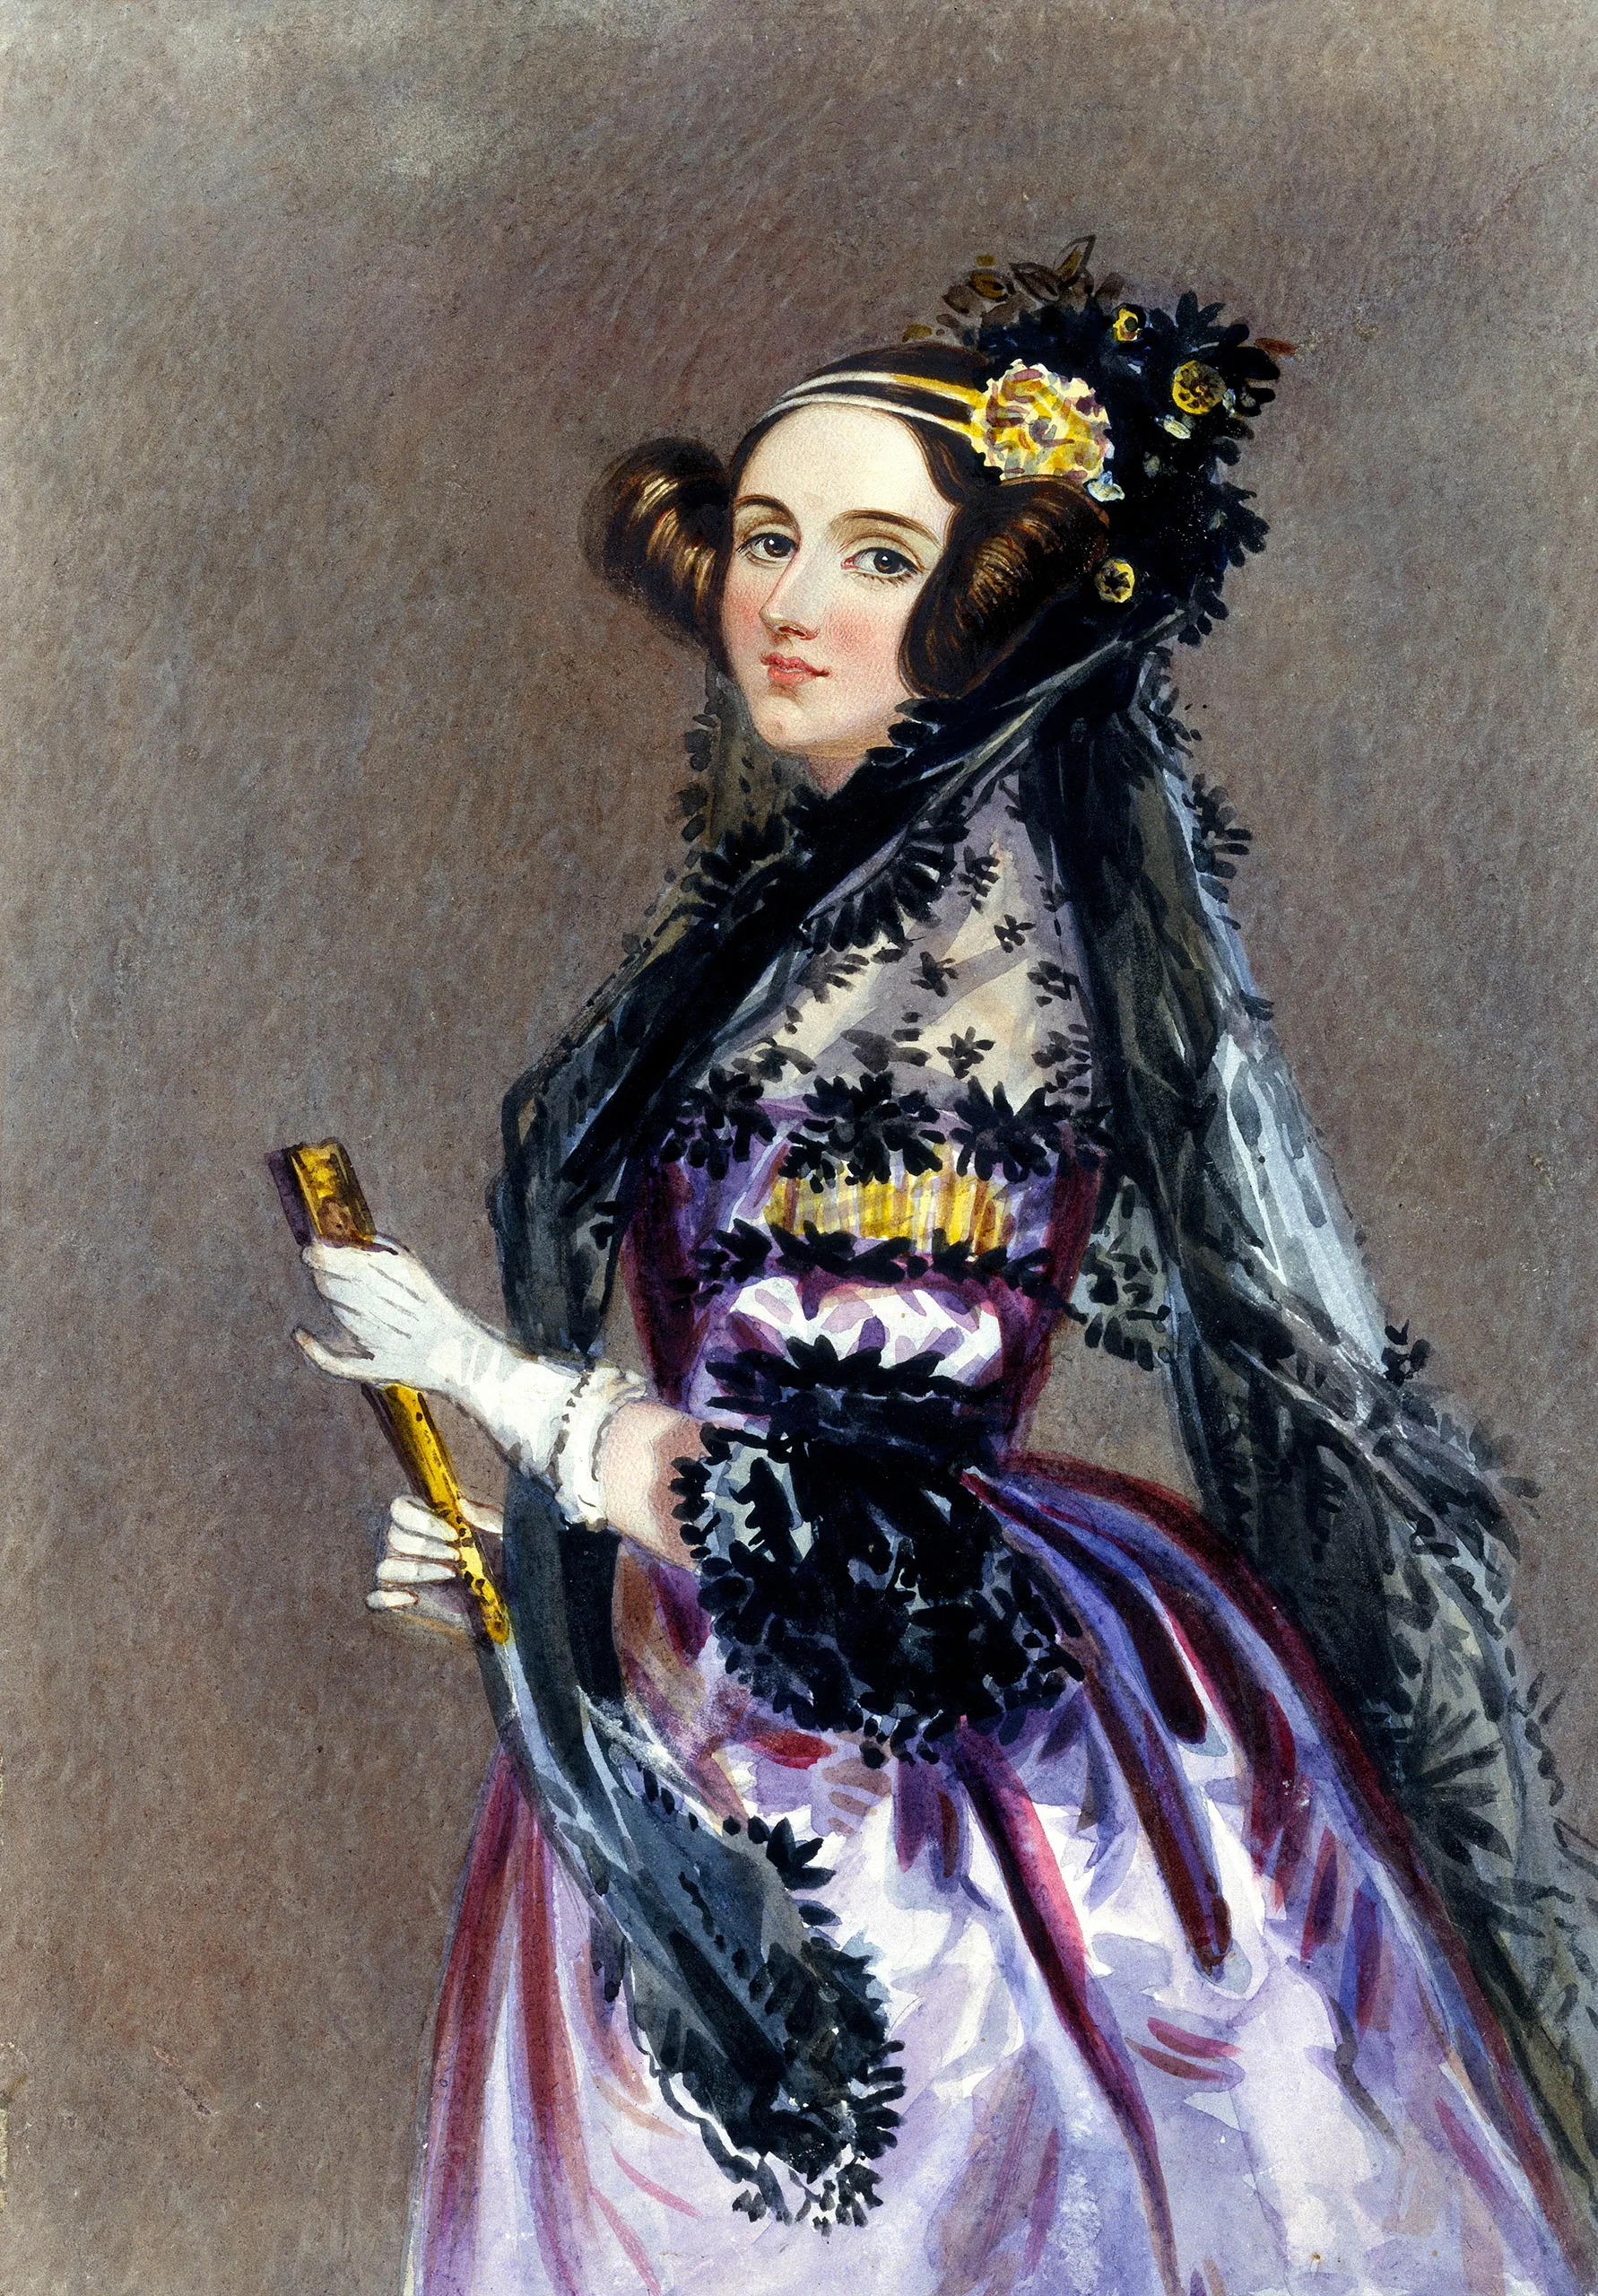
\includegraphics[height=0.7\textheight]{images/L1/lovelace.png}

    \visible<2->{\vspace{0.5ex}\scriptsize Ada Lovelace (first programmer)}
    \column{0.5\textwidth}
    \centering
    \includegraphics[height=0.7\textheight]{images/L1/hamilton.jpg}

    \visible<2->{\vspace{0.5ex}\scriptsize Margaret Hamilton (first software engineer)}
  \end{columns}
\end{frame}

\begin{frame}
  \frametitle{What is Enterprise Software?}

  \begin{itemize}
    \item \textbf{Lovalace} wrote the first algorithms for Babbage's Analytical Engine. They were \textbf{simple programs} and were meant as an intellectual exercise or proof of concept.

      \vfill

    \item \textbf{Hamilton} and her \textbf{MIT team} developed the on-board flight software for NASA's Apollo Guidance Computer. It was the \textbf{most complex} and \textbf{safest} software ever written at the time.
  \end{itemize}

\end{frame}

\begin{frame}
  \frametitle{What is Enterprise Software?}

  You are not Ada Lovelace, you are Margaret Hamilton.
  \vfill
  \begin{itemize}
    \item Software Engineers work in \textbf{teams} to solve \textbf{complex problems} with \textbf{real stakes} (potentially human lives).
    \item Complex software problems require different \textbf{architecture patterns} and \textbf{development strategies} compared to simple software.
  \end{itemize}

\end{frame}

\begin{frame}
  \frametitle{Software Engineers are Engineers}

  \begin{columns}[T,onlytextwidth]
    \column{0.7\textwidth}
    Engineers...
    \begin{itemize}
      \item Don't reinvent the wheel: use \textbf{standards} (IEEE, ISO...), \textbf{patterns} and \textbf{good practices}.
      \item Care about long-term \textbf{reliability} and \textbf{performance}.
      \item Work within \textbf{requirements} and \textbf{budgets}.
      \item Use \textbf{formal diagrams} to communicate.
      \item Build prototypes and run controlled experiments.
    \end{itemize}

    \column{0.3\textwidth}
    \centering
    \begin{tikzpicture}
      \umlclass{SoftwareEngineer}{}{}
      \umlclass[x=0,y=2]{Engineer}{}{}

      \umlinherit[geometry=-|]{SoftwareEngineer}{Engineer}
    \end{tikzpicture}

  \end{columns}

\end{frame}

\section{Block B - Project overview}
\subsection{Basic requirements}
\begin{frame}
  \frametitle{Basic requirements}
  \begin{itemize}
    \item The client wants the frontend to be a web-app.
      \begin{itemize}
        \item This is good for us. We can write one web-app instead of creating native applications for Windows, Android, iOS, etc.
      \end{itemize}
    \item We need to persist information about the users, teams, etc.
      \begin{itemize}
        \item We'll need a database.
      \end{itemize}
    \item The entire system must be performant, reliable and secure.
  \end{itemize}
\end{frame}

\subsection{Physical architecture}
\begin{frame}
  \frametitle{Physical architecture}
  We'll use a simple and battle-tested Client-Server architecture:
  \begin{figure}
    \includegraphics[scale=1]{images/L1/PhysicalArch1.pdf}
    \caption{Physical architecture high-level overview}
  \end{figure}
\end{frame}

\begin{frame}
  \frametitle{Choosing technologies}

  We'll pick the most widely used technologies for each area:
  \url{https://survey.stackoverflow.co/2025/technology/}
  \newline
  \newline
  Other decisions that need to be made:
  \begin{itemize}
    \item Client-Side Rendering vs Server-Side Rendering
    \item REST vs GraphQL
      \begin{itemize}
        \item \url{https://blog.postman.com/graphql-vs-rest/}
      \end{itemize}
  \end{itemize}
\end{frame}

\begin{frame}
  \frametitle{Physical architecture \& Used technologies}
  \begin{figure}
    \includegraphics[scale=1]{images/L1/PhysicalArch2.pdf}
    \caption{Physical architecture high-level overview}
  \end{figure}
\end{frame}

\section{Block C - Project structure \& demo}

\begin{frame}
  \frametitle{Project structure}

  Configuration files (which you can probably ignore):
  \begin{itemize}
    \item \texttt{pom.xml}: Maven project configuration and dependencies.
    \item \texttt{MainApplication.java}: Main application entry point.
    \item \texttt{config/*}: Sprint components and configuration.
  \end{itemize}

\end{frame}

\begin{frame}
  \frametitle{Project structure}

  \textbf{Important files for development:}
  \begin{itemize}
    \item \texttt{controller/*}: Web layer. This is where REST endpoints are created (one file for each resource group).
    \item \texttt{domain/*}: Domain layer. This contains a Java implementation of the domain entities (and their corresponding business logic).
    \item \texttt{repository/*}: Persistence layer. Contains Spring Data interfaces for storing/loading entities from/to the database.
    \item \texttt{handler/*}: Hooks that perform additional work on certain lifecycle events from the persistence layer.
  \end{itemize}

\end{frame}

\begin{frame}
  \frametitle{Project structure}

  \textbf{Important files for testing:}
  \begin{itemize}
    \item \texttt{test/resources/features/*}: Cucumber features (BDD).
    \item \texttt{test/java/.../steps/*}: Java implementation of steps that can be used in the feature files.
  \end{itemize}

\end{frame}

\section{Work assignment}
\begin{frame}
  \frametitle{Work assignment}

  \begin{enumerate}
    \item Make sure you have completed the "Group creation" test. Wait to get access to the "UdL-EPS-SoftArch-Igualada" GitHub organization.
    \item Clone the backend (Java) repository. Be careful \textbf{not} to clone the \textit{template} repo.
    \item Create and push new branch for your changes. You \textbf{do not} need to create a \textit{fork} of the repository.
    \item Write the basic code for the domain model classes that were assigned to you in class. You \textbf{must} use \href{https://en.wikipedia.org/wiki/Pair_programming}{pair programming}. Use the existing model classes as examples.
    \item Commit your changes with a descriptive message, and create a Pull Request.
  \end{enumerate}
\end{frame}

\end{document}
